% Cross-Layer F1 vs WER Curve (analytical noise ladder vs. measured ASR->LLM points)
% Blue series = run_cross_layer_curve.py default mode: resamples the 32-term gold list,
%   never calls the LLM, F1=1.000 at 0% WER by construction. Model, not measurement.
% Red series = the 11 measured points of tables/cross_layer_measured.tex.
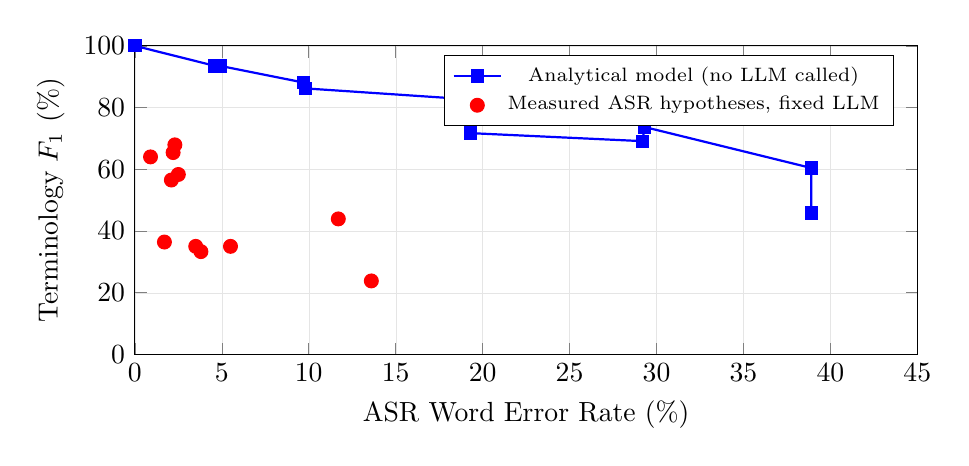
\begin{tikzpicture}
\begin{axis}[
    width=0.95\columnwidth, height=5.5cm,
    xlabel={ASR Word Error Rate (\%)},
    ylabel={Terminology $F_1$ (\%)},
    xmin=0, xmax=45, ymin=0, ymax=100,
    grid=both, grid style={line width=.1pt, draw=gray!20},
    legend pos=north east, legend style={font=\scriptsize}
]
\addplot[color=blue, mark=square*, thick] coordinates {
    (0.0, 100.0) (0.0, 100.0) (4.6, 93.5) (4.9, 93.5) (9.7, 88.1) (9.8, 86.2) (18.8, 82.8) (19.3, 71.7) (29.2, 69.1) (29.3, 73.7) (38.9, 60.4) (38.9, 45.8)
};
\addlegendentry{Analytical model (no LLM called)}

\addplot[color=red, mark=*, only marks, mark size=2.5pt] coordinates {
    (3.8, 33.3) (2.1, 56.5) (1.7, 36.4) (2.3, 67.9) (5.5, 35.0) (2.2, 65.4) (3.5, 35.0) (13.6, 23.8) (0.9, 64.0) (11.7, 43.9) (2.5, 58.3)
};
\addlegendentry{Measured ASR hypotheses, fixed LLM}
\end{axis}
\end{tikzpicture}
